% Candidate source: src-22a421a422f050bc84accae7bf41feb6903c62df04bd83f34d8267d28f49ee2e
% Source PDF SHA-256: 092e8e90dc1430ab2fa8b8ce79e072e317559e6bef29f1cb7461e9423925ec31
% PDF page 1 (printed page 262), question 17.
% Redraw follows visible/hidden edges; perspective is schematic, not to scale.
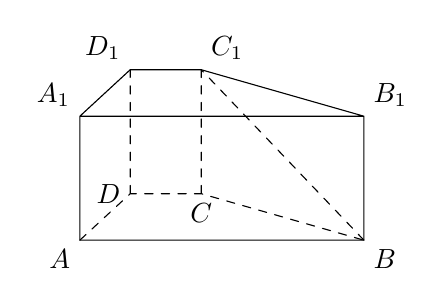
\begin{tikzpicture}[line cap=round,line join=round,x=0.82cm,y=0.82cm]
  \coordinate (A) at (0,0);
  \coordinate (B) at (4.4,0);
  \coordinate (D) at (0.78,0.72);
  \coordinate (C) at (1.88,0.72);
  \coordinate (Aone) at (0,1.92);
  \coordinate (Bone) at (4.4,1.92);
  \coordinate (Done) at (0.78,2.64);
  \coordinate (Cone) at (1.88,2.64);

  % Hidden base and rear vertical edges.
  \draw[dashed] (A)--(D)--(C)--(B) (D)--(Done) (C)--(Cone);
  % Visible lower/front and upper prism edges.
  \draw (A)--(B) (A)--(Aone)--(Bone)--(B)
        (Aone)--(Done)--(Cone)--(Bone);
  % The marked space diagonal BC_1 is dashed in the source.
  \draw[dashed] (B)--(Cone);

  \node[below left] at (A) {$A$};
  \node[below right] at (B) {$B$};
  \node[below] at (C) {$C$};
  \node[left] at (D) {$D$};
  \node[above left] at (Aone) {$A_1$};
  \node[above right] at (Bone) {$B_1$};
  \node[above right] at (Cone) {$C_1$};
  \node[above left] at (Done) {$D_1$};
\end{tikzpicture}
